% ceci est le brouillon de la suite du projet 
\begin{table}[htbp]
    \small
    \centering
    \begin{tabularx}{\linewidth}{l|p{1.7cm}|X|X}
        \toprule
        \textbf{identifiants} & \textbf{sujets} & \textbf{dates} & \textbf{page} \\
        \midrule
         Valla\_Adn & Commentaires pauliniens & 1505 & \href{https://api.digitale-sammlungen.de/iiif/image/v2/bsb11059298_00082/full/1134,/0/default.jpg}{f.49v}, \href{https://api.digitale-sammlungen.de/iiif/image/v2/bsb11059298_00083/full/1134,/0/default.jpg}{f.50r} \\
        Okolampadius\_Rom & Commentaires pauliniens & 1525 & \href{https://www.e-rara.ch/download/webcache/1000/2122892}{p.5}, \href{https://www.e-rara.ch/download/webcache/1000/2123062}{p.90}\\
        Daneau\_1\_Tim\_C5& Commentaires pauliniens & 1577 & \href{https://www.e-rara.ch/download/webcache/1000/2013217}{p.305}, \href{https://www.e-rara.ch/download/webcache/1000/2013288}{p.376}\\
        Aretius\_1\_Tim & Commentaires pauliniens & 1580 & \href{https://www.e-rara.ch/download/webcache/1000/6289349}{p.9}, \href{https://www.e-rara.ch/download/webcache/1000/6289387}{p.47}\\
        \midrule
        Pellican\_Ct & Cantique~des Cantiques & 1582 & \href{https://www.e-rara.ch/download/webcache/1000/8471143}{p.266r} \href{https://www.e-rara.ch/download/webcache/1000/8471152}{p.270v} \\
        De\_Jon\_Gen & Genèse & 1603 & \href{https://www.e-rara.ch/download/webcache/1000/21301625}{p.17}, \href{https://www.e-rara.ch/download/webcache/1000/21301657}{p.49} \\
        \midrule
        Philelphi\_Inst & poésie & 1544 & \href{https://www.e-rara.ch/download/webcache/1000/2207608}{p.2}\\
        Beatini\_Ad\_Clem & poésie & 1544 & \href{https://www.e-rara.ch/download/webcache/1000/2207529}{p.2}\\
        Palingenus\_Zod & poésie & 1605 & \href{https://www.e-rara.ch/download/webcache/1000/13982576}{p.188}, \href{https://www.e-rara.ch/download/webcache/1000/13982731}{p.343}\\
        \bottomrule
    \end{tabularx}
    \caption{Corpus test lemmatisation }
\end{table}


\subsection{Les humanités numériques et les sciences humaines}

% considération épistémologique 
%la différence remonte au final au première réflexion épistémologique
Qu'est ce qu'une science humaine ? 
1. comprendre et expliquer 
=> les sciences humaine = comprendre = l'importance du sens
=> expliquer dépendant du domaine de la causalité 

Or l'emploie de modèle de langue et de procédé comme le topic modeling rebatte les cartes, car ils fournisse des résultat dont la causalité directe est insaisissable.

(opacité épistémologique) 
et donné des résultat par des corrélation = le reflet d'une certain réalité statistique qui permet de classer des mots les un par rapport au aux autres mais sans que la signification du mot soit prise en compte. Cette pratique est ainsi  ce que P. Huneman décrit comme "un traitement des mots sans compréhension"(p.206). Même si la formulation est forte elle n'en souligne pas moins une réalité : l'intervention dans la machine dans la recherche ne peut pour l'instant se suppléer à  l'analyse humaine qui permet de tirer les conclusions définitives. En faisant entrer des variables "opaque" dans le processus de recherche l '

-opacité des données, pertes de la valeur de la causalité ou profit de la corrélation statistique clé des résultats dit de "prédiction". Conséquence importance de décrire le processus , chaîne de traitement, donnée dans l'objectif d'avoir une expérience productible. (lolisme). que la réflexion sur le commentaire à Timothée forme la première étape de notre réflexion est devra est élargie à un corpus beaucoup plus vaste dans la suite du projet. 
%%%%%%%%%%%%%%%%%%%%%%%%%%%%%%%%%%%%%



https://www.e-rara.ch/zuz/content/zoom/1298021 (forcher + full greek)
https://www.e-rara.ch/zuz/content/zoom/1298050 (forcher + full greek)
Conclusion = si on veut lemmatiser sans y passer sa vie, il faut que l'ocr sont très bon. 
https://www.e-rara.ch/bau\_1/content/zoom/5087560

Lorsque cela était pertinent on a repris les documents de teste de l'OCR pour le teste de lemmatisation, afin de tirer avantage au maximum des données produites. 
Corpus italique = corpus de poésie
Okolampadius = paulinien non vue
Nicolas de Lyre = out of domaine. 

Il faut encore clarifier définitivement le test fait sur les doc in domaine et ceux out of domaine.


le script nécessite d'adapter aux nouveaux cas de figures qui ne manqueront pas d'apparaître au fur et à mesure de l'accroissement du corpus. On peut cependant espérer que la standardisation du système abréviatif soit suffisante pour arriver à une situation de pleine efficacité après avoir testé le script sur une quantité de donnée suffisante.\par 
\FloatBarrier

Le traitement de donnée en néolatin est un des volet du projet FNS sur l'exégèse de Paul~\cite{exegesisofPaul_2023}Lemmatisation L'objectif est de traiter un large corpus de commentaires pauliniens du XVIe siècle accessibles dans des imprimés numérisés. La finalité du projet est de créer une bibliothèque digitale et fournir des outils de travail pour un traitement digitale du corpus paulinienne. Le travail suivant résume la première étape du projet concernant la création d'OCR, les choix d'annotations effectués lors de l'extraction des données et de la lemmatisation.

\centering
    \small
        \begin{tabular}{|c|c|c|c|c|c|}
        \hline
        \textbf{Corpus} & \textbf{variables}  & \textbf{Gallicopora} & \textbf{Lambertus-10} & \textbf{Lambertus.03} & \textbf{nfd\_best.mlmodel} \\
        \hline
        \multirow{4}{*}{\textbf{Corpus Général}}
         & CAcc & 98.16 & 98.95 & \textbf{99.02} & 98.93\\ 
         & CER & 1.84 & 1.05 & 0.98 & 1.07\\
         & WAcc & 91.74 & 95.87 & \textbf{96.12} & 95.66 \\
         & WER & 8.25 & 4.12 & 3.87 & 4.33 \\
        \hline
        \multirow{4}{*}{\textbf{Corpus exégèse complet}} 
         & ACC & 97.61 & 98,89 & \textbf{98.96} & 98.95\\
         & CER & 2.39 & 1.11 & 1.04 & 1.05\\
         & WACC & 89.56 & 94.62 & \textbf{95.02} & 94.76\\
         & WER & 10.43 & 5.38 & 4.97 & 5.23 \\
        \hline
        \multirow{4}{*}{\textbf{corpus exégèse Daneau}}
         & ACC & 97.93 & \textbf{99.1} & 99.08 & 99.08\\
         & CER & 2.07 & 0.90 & 0.92 & 0.92\\
         & WACC & 91.08 & \textbf{96.09} & 95.98 & 95.73 \\
         & WER & 8.19 & 3.90 & 4.01 & 4.26 \\
        \hline
        \multirow{4}{*}{\textbf{italique latin}} 
         & ACC & 97.13 & 99.01 & 99,23 & \textbf{99.31}\\
         & CER & 2.87 & 0.99 & 0.77 & 0.69 \\
         & WACC & 84.59 & 96.07 & 96.22 & \textbf{96.60} \\
         & WER & 15.4 & 3.92 & 3.77 & 3.39 \\
        \hline
        \hline
        \multirow{4}{*}{\textbf{exégèse inconnue + Genesis}} 
        & ACC & 97.39 & 98.40 & 98.56 & \textbf{98.95}\\
        & CER & 2.61 & 1.60 & 1.44 & 1.05\\
        & WACC & 86.19 & 90.14 & 91.11 & \textbf{93.35}\\
        & WER & 13.8 & 9.85 & 8.88 & 6.64 \\
        \hline
        \multirow{4}{*}{\textbf{exégèse inconnue type paulinienne}} 
        & ACC & 97.95 & 98.83 & 98.96 & \textbf{99.14}\\
        & CER & 2.05 & 1.17 & 1.04 & 0.86\\
        & WACC & 88.32 & 92.0 & 93.06 & \textbf{94.51}\\
        & WER & 11.67 & 7.99 & 6.93 & 5.48 \\
        \hline
        \end{tabular}
        \caption{Résultats des 4 modèles sur différent jeu de test. Les meilleures resultat sont indiqués en gras. L'extraction des données suit la méthode décrite dans le dépôt GitHub \href{https://github.com/FoNDUE-HTR/kamiCLI}{kamiCLI} avec l'application d'un script python pour le calcule finales des moyennes. 
        *les résultats ci-dessus sont des moyennes arrondies à la seconde décimale}
        \label{tab:wide_table}
    \end{table*}

    Dans le présent travail le découpage en verset qui structurera les comparaisons du topic modeling à été fait manuellement. Cette tâche devra être automatisée à l'avenir. L'expérience précédente permet tout de même de tirer une conclusion sur la direction à prendre dans cette nouvelle problématique. Il n'est pas pertinent d'essayer de l'intégrer lors de l'océrisation du document.
-ajout à la main et variance dans le corpus. La solution est probablement d'intégrer ce découpage dans le document en TEI. 
-mais variance, entre le texte des versets et le textes cités dans les commentaires donc 
Une solution comme celle-ci pourrait être interessante à voir.
Solution en deux étapes:
1. travailler la reconnaissance des variables sur un doc en txt. 
https://www.wisecube.ai/blog/named-entity-recognition-ner-with-python/
ou un outil de type chatgpt.
2. une fois que les éléments sont tagger dans le txt. Les versets variants sont balisés et on peut avec un script basé sur des mots identiques en python tagger ces mêmes versets dans la tei. 
Le passage par le txt permet de travailler sur un document simplifié, notamment si une étape de tokenization est necessaire, ce qui sera certainement le cas.


\subsection{Pipe line pour le developpement Web}
Le schéma ci dessous décrire les étape à suivre en vue du déploiement Web du projet sous forme d'une bibliothèque digitale. 

\begin{figure*}[b]
    \subsection{Pipeline pour le developement Web}
    \centering
    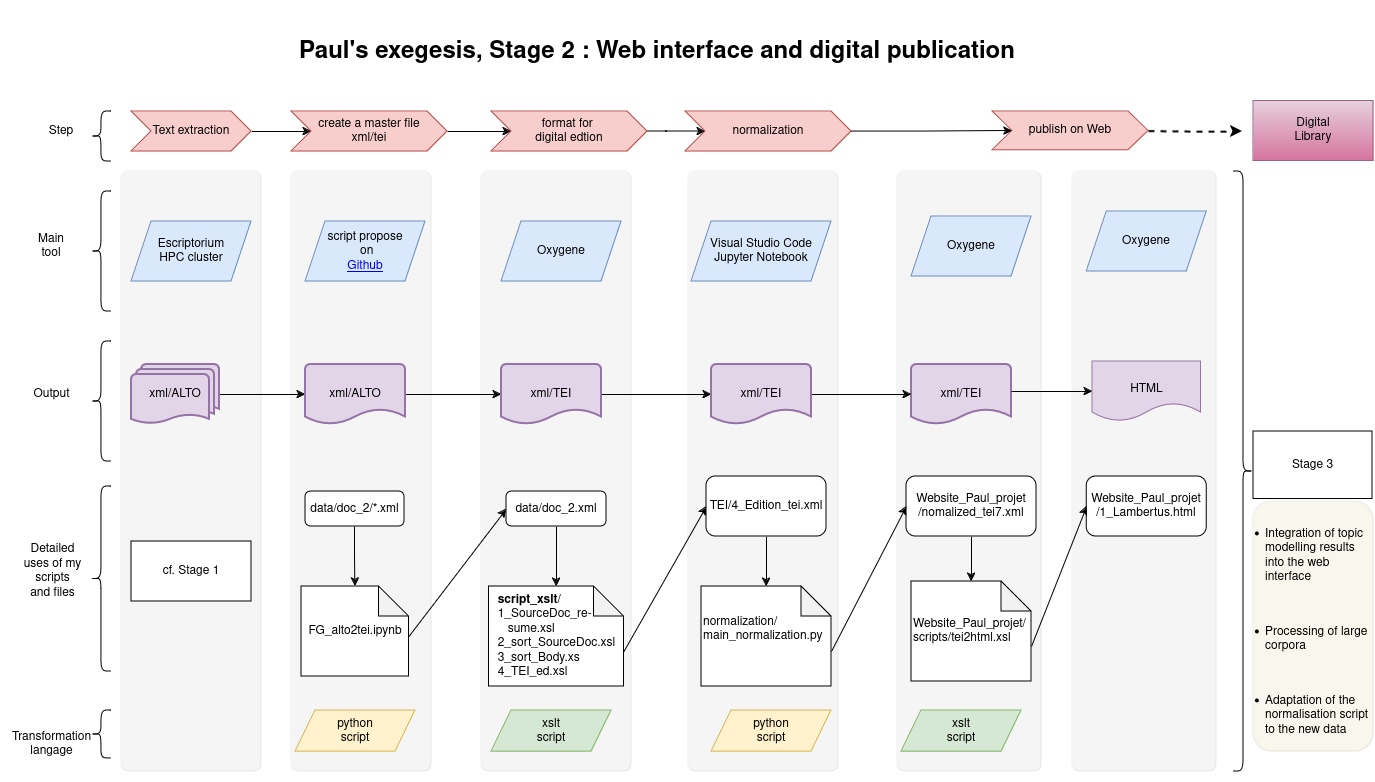
\includegraphics[width=1.1 \linewidth]{Paul_Pipeline.png}
    \caption{On trouvera toutes les informations relative à la Pipeline sur le dépot GitHub : \href{https://github.com/FourbeFlo/PipeLine-for-Web-interface}{PipeLine-for-Web-interface}}
    \label{fig:large_graphic4}
\end{figure*}
\FloatBarrier
\clearpage
\newpage


\todo[inline]{Moi je dirai pas (beaucoup) plus que ça} mooooooooooooooooooooort!


\subsection{recommandation pour la suite du projet}
Avec une chaîne de traitement des données fonctionnelle, l'enjeu est d'examiner un très grand nombre de texte, afin de pouvoir bénéficier pleinement de l'approche computationnelle du big data. nous préconisons les suivants :
\begin{itemize}
    \item OCR : segmentation et océrisation
\end{itemize}
    la présence d'échantillons variants peut faire chuter les performances de l'OCR. Il faudra donc rester attentif au résultat obtenu et considérer le temps de correction manuelle à apporter si besoin. 
\begin{itemize}
    \item amélioration du modèle de lemmatisation avec l'insertion de nouvelles données
\end{itemize}
Il faut un plan de lemmatisation pour assurer une anontation régulière des données, au fur et à mesure de l'élargissement du corpus. Pour avoir un modèle de lemmatisation efficace, nous préconisons de selectionner des échantillions parmi les textes des les collaborateurs. Cette pratique augmentera d'autant l'efficacité du modèle sur ces document ce qui sera profitable pour le topique modeling.   
\begin{itemize}
    \item protocole de nommages
\end{itemize}
 L'établissement d'un corpus large nécessite un protocole de nommage défini en amont de la recherche. Le protocole doi être appliqué par tous les collaborateurs du projet.
 \begin{itemize}
    \item La reconnaissance d'entités nommés : le problème des versets
\end{itemize}
Les versets qui structurent le texte biblique doivent être localisés dans le corps du texte. Pour l'instant nous avons décidé de les intégrer manuellement dans la tei.Mais des solutions automatisées méritent d'être envisagée à l'avenir.